\documentclass[class=article, crop=false]{standalone}
\usepackage[utf8]{inputenc}


\usepackage{amsfonts}
\usepackage{amsmath}
\usepackage[english]{babel}
\usepackage{booktabs}
\usepackage{caption}
\usepackage{graphicx}
\usepackage{import}
\usepackage{multicol}
\usepackage{multirow}
\usepackage[subpreambles=false]{standalone}
\usepackage{subcaption}
\usepackage{tikz}

\usepackage[linesnumbered,ruled,vlined]{algorithm2e}
\newcommand\commentfont[1]{\footnotesize\ttfamily\textcolor{blue}{#1}}
\SetCommentSty{commentfont}

\usepackage[backend=biber]{biblatex}
\addbibresource{references.bib}

\usepackage{geometry}
\geometry{
   a4paper,
   left=20mm, right=20mm,
   top=20mm, bottom=25mm
}
 
\usepackage{hyperref}
\hypersetup{
  colorlinks=true,
  linkcolor=blue,
  citecolor=black,
}

\usepackage{pgfplots}
\pgfplotsset{compat=1.3}
 
 
\setlength{\tabcolsep}{2pt} % Default value: 6pt
\renewcommand{\arraystretch}{1} % Default value: 1


\begin{document}




\section{Explanation of important concepts}
\label{sec:app_imp_concepts}
% \explain different transformations (rigid...), centering, rotating..
\begin{description}
    \item[Rigid deformation] Deformation describes the transformation of an object from an initial to some final geometry. In contrast to non-rigid deformation, a rigid deformation does not change the position and orientation of the object relative to the internal reference frame. Rotation around an axis is an example of a rigid operation that changes the configuration of the points relative to the external but not to the internal reference frame. Translation is another rigid transformation because it only affects the external reference frame, as the points within the object are all moved along parallel paths to the axis.
    \import{}{import/rigid.tex}
    
    \item[Non-rigid deformation] Non-rigid deformations can affect points within the object relative to both the internal and external reference frame. Distortion is an example of a non-rigid operation that changes the spacing of points within the object and consequently changes the object's overall shape. Dilation or scaling is another non-rigid operation that changes the object's volume, but differently from distortion, retains the same shape.
    \import{}{import/nonrigid.tex}
    
    % \item[Intrinsic/extrinsic deep learning] Extrinsic deep learning methods treat the geometric data as Euclidean data with zero curvature, whereas intrinsic deep learning treats the object as manifolds with non-zero curvature.
    % \import{}{import/ex-intrinsic_dl.tex}
    
    \item[Shape descriptor] A shape descriptor characterizes the local geometry of the surface. In other words, they describe a point's role on the surface. Examples for shape descriptors are the Gaussian curvature $K(x) = \kappa_1(x)\kappa_2(x)$ and the mean curvature $H(x) = \kappa_1(x)+\kappa_2(x)$. Good shape descriptors are robust to noise in the triangulation and against small deformations. They should also be invariant under rigid transformation and other isometries. \cite{stanfod_iso}
    
    \item[Heat Kernel Signature] The Heat Kernel Signature (HKS) is a popular shape descriptor. It is related to the eigenvalues and eigenfunctions of the Laplace–Beltrami operator.
    % If we define $k_t(x,y)$ as the solution to the heat equation
    
    % \begin{equation}
    %     u_t = u
    % \end{equation}
    For a fixed time $t$, it is defined as 
    \begin{equation}
        HKS(x) = k_t(x,x) = \sum_{i} e^{-\lambda_i t}\phi_i(x)^2,
    \end{equation}
    where $\lambda_i$ is the i-th eigenvalue and $\phi_i$ the i-th eigenfunction of the Laplace-Beltrami operator.
    The time describes how locally or globally the shape is captured from a given point (see Figure \ref{fig:hks_dragon}).
    
    There are different shape descriptors, such as the Wave Kernel Signature (WKS) similar to HKS but based on the Schrödinger wave equation. Each has its advantages depending on the application, but both are invariant to isometric transformations and can be computed efficiently.
    Furthermore, HKS is also stable under small perturbations to the shape.
    \import{}{import/hks_dragon.tex}
    
    \item[Manifold meshes] Generally speaking, a manifold is a topology that locally resembles Euclidean space. In computer graphics, often, triangular meshes are used as they are the simplest form of polygon meshes and require fewer computations for computer graphical operations. Many applications require the reconstructed triangular mesh surface to be a watertight manifold surface with correct topology. Watertightness is fulfilled if the mesh does not have holes or missing triangles. Formally, a mesh is manifold if every edge in the mesh is either a boundary edge or a manifold edge, whereas a boundary edge is part of exactly one face and a manifold edge of two faces. Moreover, it does not include non-manifold vertices, i.e. vertices where the corresponding star (= union of all incident faces) is not connected when removing the vertex. See Figure \ref{fig:non-manif-e-v} for an illustration of a non-manifold vertex and non-manifold edge.
    Fixing the mesh to be manifold or watertight is called mesh healing or mesh repairing.
    \end{description}
    
    
\vspace{0.05\linewidth}

\begin{figure}[h]
    \centering
    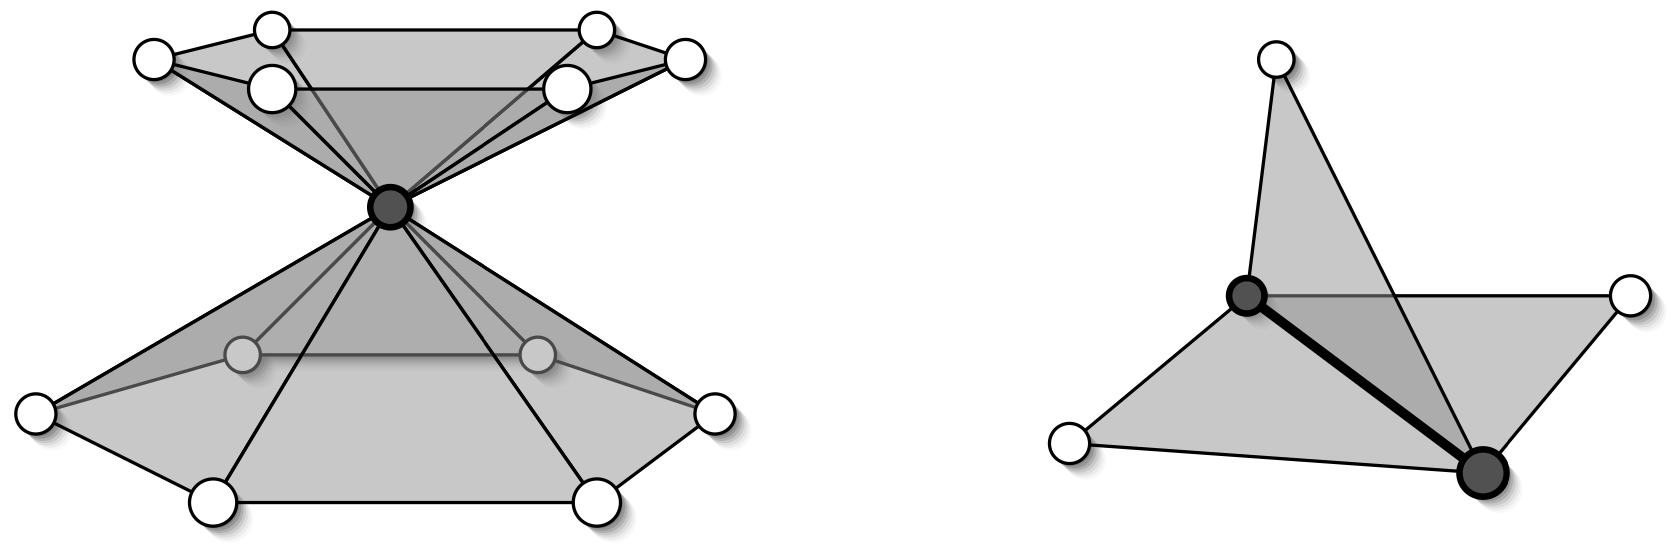
\includegraphics[width=0.4\linewidth]{thesis/appendices/import/imgs/non-manif-e-v.png}
    \caption{\textbf{Non-manifold geometry.}
\small Non-manifold vertex (left), non-manifold vertex (right). Image from \cite{Botsch2010}.
geed}
    \label{fig:non-manif-e-v}
\end{figure}
\vspace{0.05\linewidth}
    


\section{Background for choice of the approach}
\label{sec:app_approach_choice}
\subsection{Network}
The project started with exploring different networks that can tackle the problem of 3D landmark detection. This phase also led to insights regarding networks that do not work well for the problem. PointNet is one of the earliest and more straightforward model architecture that operates on point clouds was a straightforward choice. The first attempts involved the Pytorch implementation of the extension of PointNet, called PointNet++. However, experiments on this network were difficult because of the very high memory consumption of the network architecture, indicating poor scalability. Even for decimated meshes, the input images were still too big for the approach of predicting point-wise activations per landmark channel.

The next attempt to tackle the problem was MeshCNN, which showed better scaling properties and lower memory consumption in our experiments. The motivation to use a network that processes meshes directly instead of point clouds is that meshes include additional surface information that can better capture the surface structure. Specifically, MeshCNN combines specialized convolution and pooling layers that operate on the edges of the mesh. While the first results of a network that performs direct coordinate regression were promising, one big drawback prevents using MeshCNN in practice: the network requires mesh watertightness or manifoldness. Repairing the meshes is usually a manual task in a 3D computer graphics software such as Blender \cite{blender} or Meshlab \cite{meshlab} that cannot easily be automized inside a preprocessing pipeline. Therefore, it is not feasible to apply MeshCNN on unseen meshes, e.g. the meshes of the control samples from the Radboudumc data set.

\subsection{Direct coordinate regression vs point-wise regression}
\label{sec:coord_reg_vs_pw_reg}
A straightforward way to learn the XYZ coordinates of landmarks is to build a regression network that predicts the coordinates directly. However, experiments performed on the MeshCNN network suggested that this approach tends to overfit the average face structure observed in the training set, as opposed to learning surface-based features (see Figure \ref{fig:meshcnn_res}). Notably, the set of possible predictions also includes all points in space, not restricted to points on the mesh surface. A point-wise approach circumvents this problem by predicting a score for each point, thus only allowing landmark predictions located on the surface of the mesh. Besides, a point-wise approach enables the learning of point clusters that represent a region in proximity of a landmark.
\import{}{import/meshcnn_res.tex}


% write about manual landmark annotations, how long it takes, which landmarks are easy, which hard...

\section{Manual annotation}
\label{sec:app_manual_annotation}
We quickly reach a threshold where not the approach and network architecture but the poor annotation quality limit detection performance. Thus, 307 Headspace samples are manually annotated in 3DMedX. The samples are labelled by two annotators, each annotating roughly half of them. Therefore, it is to be expected that there is a small interobserver variability among the annotations. Specific samples are left out if they meet one of the criteria: Firstly, the photo is left out if the subject has a moderate or heavy beard because it is hard to define the correct landmark positions of pogonion, left cheilion and right cheilion for such subjects. Secondly, the photo is left out if no texture information is available for the corresponding mesh. The third criterion is if artefacts in the mesh prevent the annotator from properly labelling one of the landmarks. This can happen in rare cases where the mesh has a prominent chin hole.
After the annotation process, the average variability between the Headspace and manual labels is measured at 3.81mm. This number suggests that there is indeed an inaccuracy in the Headspace labels that can prevent the model from learning the correct facial features.
% ones with beard left out
% some more difficult than others
% saved as coordinate format
% variability within human and between two annotators


\section{Results details}
\label{sec:app_results}
\begin{table*}[!htbp]
\captionof{table}{\textbf{Maximum errors for Table \ref{table:ref_hks}: Refinement network assessment and HKS features.}
    }
\label{table:ref_hks_max}
\begin{tabularx}{\textwidth}{l|c|c|c}
\toprule
 & \multicolumn{3}{c}{Maximum error in mm} \\\cmidrule(lr){2-4}
Landmark               & \hspace{0.3cm}Initial Network (XYZ)\hspace{0.3cm}\hspace{0.5cm}&\hspace{0.3cm} Refinement Network (1)\hspace{0.3cm}  & \hspace{0.3cm}Initial Network (HKS) \hspace{0.3cm}    
\\
\midrule
Pogonion               & 12.78 & 8.82 & 110.15\\
Nasion                 & 5.02  & 3.16 & 7.68\\ %\pm
Pronasale              & 5.78  & 5.07 & 7.74\\
Alar curvature (right) & 4.89  & 6.58 & -\\
Subnasale              & 6.94  & 5.97 & 7.53 \\
Alar curvature (left)  & 6.13  & 11.05 & - \\
Exocanthion (right)    & 8.94  & 8.71 & 10.27\\
Endocanthion (right)   & 6.56  & 6.57 & 8.84\\
Endocanthion (left)    & 7.73  & 9.39 & 7.73\\
Exocanthion (left)     & 9.26  & 9.20 & 11.36\\
Cheilion (right)       & 10.20 & 9.84 & 44.81\\
Cheilion (left)        & 8.06  & 8.37 & 16.82\\
\bottomrule
total & \textbf{12.78} & \textbf{11.05} & \textbf{110.15}
\end{tabularx}
\end{table*}

\begin{table*}[!htbp]
\captionof{table}{\textbf{Maximum errors for Table \ref{table:horizflip_rgb}: Horizontal flipping and color features.}}
\label{table:horizflip_rgb_max}
\begin{tabularx}{\textwidth}{l|c|c|c}
\toprule
 & \multicolumn{3}{c}{Maximum error in mm} \\\cmidrule(lr){2-4}
Landmark               & \hspace{0.5cm}Initial network\hspace{0.5cm} &  \hspace{0.5cm}Refinement network (1)   \hspace{0.5cm} & \hspace{0.5cm} Refinement network (2)  \hspace{0.5cm}
\\
\midrule
Pogonion               & 9.31  & 8.21 & 8.21 \\
Nasion                 & 6.06 & 7.87 & 10.12\\  
Pronasale              & 5.38 & 4.04 & 4.03\\
Alar curvature (right) & 5.42 & 7.58 & 8.60\\
Subnasale              & 4.06 & 5.36 & 4.28\\
Alar curvature (left)  & 5.00 & 3.89 & 5.27\\   
Exocanthion (right)    & 6.96 & 6.10 & 5.01\\ 
Endocanthion (right)   & 8.57 & 7.15 & 5.58\\ 
Endocanthion (left)    & 8.06 & 7.93 & 6.47\\
Exocanthion (left)     & 6.48  & 8.65 & 9.74\\
Cheilion (right)       & 15.26 & 7.25 & 7.25\\
Cheilion (left)        & 15.48 & 11.20 & 6.42\\

\bottomrule
total & \textbf{15.48} & \textbf{11.20} & \textbf{10.12}
\end{tabularx}
\end{table*}

\end{document}